% !TEX root = ../thesis_main.tex
\chapter{Prior Ultrafast Spectroscopy Studies of SWCNTs}

\section{Inter-band and Intra-band Recombination Dynamics}


Ostojic et al.\ (2004) presented an early work regarding the carrier recombination dynamics of carbon nanotubes \cite{ostojic2004interband}. They conducted wavelength-dependent, degenerate pump-probe measurements using an optical parametric amplifier with a time resolution of $\sim$150 fs (See Section \ref{section:opa} for details regarding the function of optical parametric amplifiers) whereby the pump and probe have the same photon energy. The sample they studied consisted of a dispersion of HiPCo SWCNTs (See Sections \ref{section:cnt_synthesis} and \ref{section:dispersion_swcnt} for details).

\begin{figure}[ht]
	\centering
	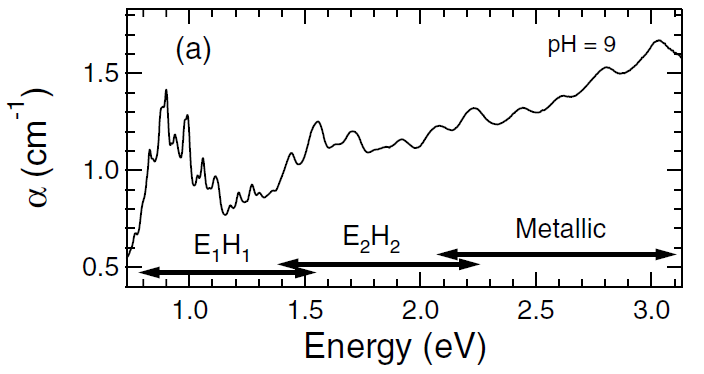
\includegraphics[scale=0.7]{images/chapter_prior_works/abs_gordana}

	\caption{Optical absorption spectrum of dispersed HiPCo SWCNTs studied by Ostojic et al.\ (2004). The spectrum contains optical resonances associated with semiconducting nanotubes which include $E_{11}$ in the region denoted as $E_{1} H_{1}$ as well as  $E_{22}$ in the region labeled as $E_{2} H_{2}$. The remaining resonances in the Metallic region come from the $E_{11}$ resonances of metallic nanotubes. Reproduced and modified from Ref.\ \cite{ostojic2004interband}.}
	\label{fig:abs_gordana}
\end{figure}


Figure \ref{fig:abs_gordana} shows the optical absorption spectrum of their sample which indicates the presence of many different chiralities, including both metallic and semiconducting nanotubes. The spectral region spanning $E_{1} H_{1}$ contains optical resonances associated with the $E_{11}$ transition occurring in semiconducting nanotubes. The region defined as $E_{2} H_{2}$ contains $E_{22}$ transitions of semiconducting nanotubes. Finally, the region defined as Metallic exhibits the remaining $E_{11}$ resonances emerging from metallic nanotubes.

\begin{figure}[ht]
	\centering
	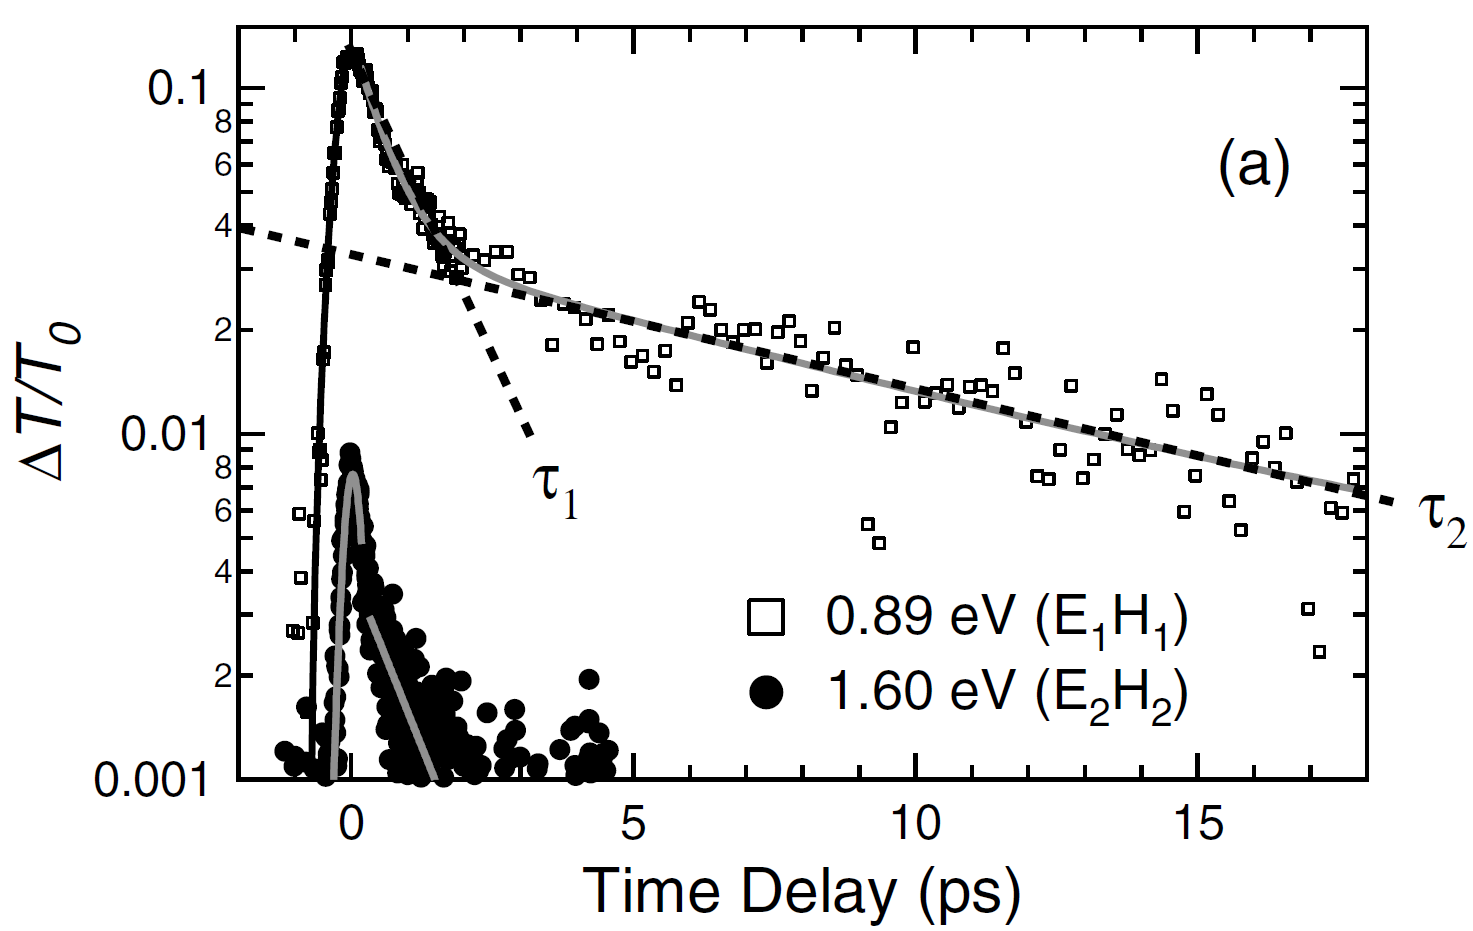
\includegraphics[scale=0.3]{images/chapter_prior_works/dtt_gordana}
	\caption{Differential transmission data at photon energies 0.89 eV (white squares) and at 1.60 eV (black circles) obtained from degenerate pump-probe measurements. At 1.60 eV, only a single exponential decay process associated with intra-band relaxation is observed. At 0.89 eV, a bi-exponential decay occurs. The fast and slow components of the bi-exponential decay are associated with intra-band and inter-band dynamics respectively. Reproduced and modified from Ref.\ \cite{ostojic2004interband}}
	\label{fig: abs_gordana}
\end{figure}

The observed carrier dynamics showed a clear wavelength dependence as shown in Figure \ref{fig:dtt_ph_gordana}. For pumping and probing within the $E_2 H_2$ region, carrier was best described by a single exponential decay process which was interpreted as intra-band relaxation to lower-energy states. In contrast, a bi-exponential decay process was observed when pumping and probing in the $E_1 H_1$ region. The initial, fast decay was interpreted as intra-band relaxation. However, the following slow exponential decay process was interpreted as inter-band relaxation. At the time of publication, this slow exponential decay process had not been observed before.

Ostojic et al.\  also note that for any chosen wavelength in their degenerate pump-probe study, some nanotubes are resonantly excited whereas others are photo-excited in a non-resonant fashion. This can affect the observed carrier decay dynamics. Figure \ref{fig:wl_dep_gordana} demonstrates this behavior. When photo-exciting the sample at an optical resonance, the ratio between the slow and fast decay times reaches a local maximum. In contrast, when pumping at spectral regions that do not exhibit a well-defined resonance, this ratio diminishes.

\begin{figure}[ht]
	\centering
	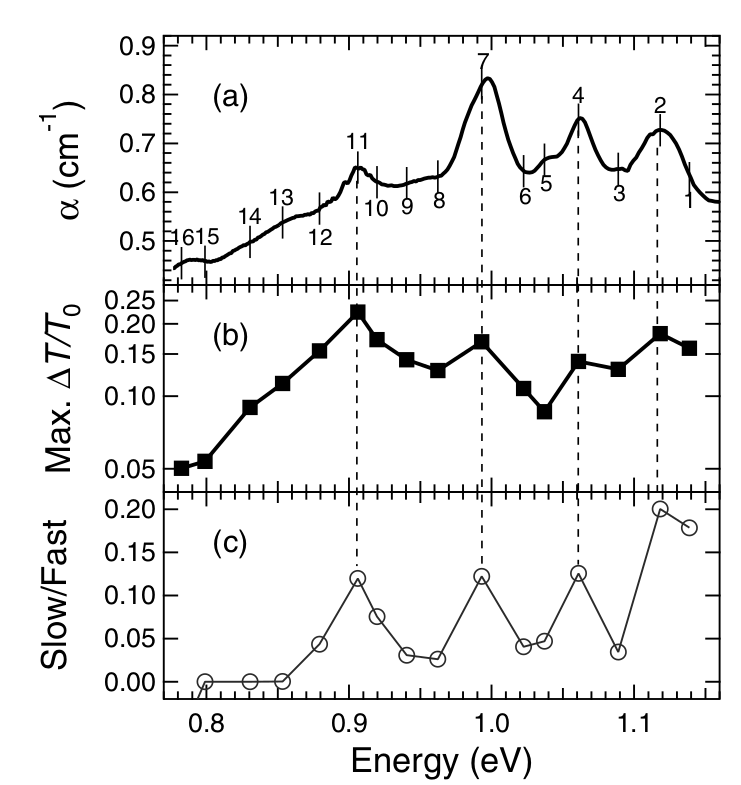
\includegraphics[scale=0.3]{images/chapter_prior_works/wavelength_dependence_gordana}
	\caption{(a) Optical absorption spectrum of the HiPCo SWCNT dispersion. The labeled positions indicate photon energies at which pump-probe measurements were taken. (b) Maximum differential transmission recorde at each measured photon energy. Differential transmission appears to reach a local maximum when the photon energy matches an optical resonance. (c) Ratio between the slow and fast decay times at each measured photon energy. The slow decay time reaches a local maximum when pumping at an optical resonance. Reproduced and modified from Ref.\ \cite{ostojic2004interband}}
	\label{fig:wl_dep_gordana}
\end{figure}

Hence, resonant excitation enhances the appearance of inter-band recombination dynamics. However, non-resonant excitations are more associated with the fast intra-band dynamics. This suggests that the reported decay times only yield statistical averages of the carrier lifetime of the ensemble of all nanotubes that have optical resonances at energies less than or equal to the pump photon energy. Furthermore, they acknowledge that they did not observe a clear correlation between the power of the optical pump and the observed carrier decay times. This excludes the observation of any nonlinear, nonradiative recombination mechanisms such as Auger recombination or exciton-exciton annihilation.

Decreasing the pH of the sample was observed to suppress optical absorption peaks, especially those occurring at lower photon energies as shown in Figure \ref{fig:ph_abs_gordana}. Correspondingly, the presence of the slow exponential decay process also diminished as shown in Figure \ref{fig:dtt_ph_gordana}. These effects were understood as a consequence of the Burstein-Moss effect. In other words, H$^+$ ions of the acidic aqueous suspension dope suspended SWCNTs by accepting negatively-charged carriers. This positions the Fermi level primarily within the valence band for nanotubes with larger diameters due to their smaller acceptor binding energies associated with their smaller effective masses.  As a result, the appearance of an inter-band absorption peak diminishes which subsequently removes the possibility of enhancing the occurrence of the inter-band relaxation by photo-exciting at well-defined optical resonances.

\begin{figure}[ht]
	\centering
	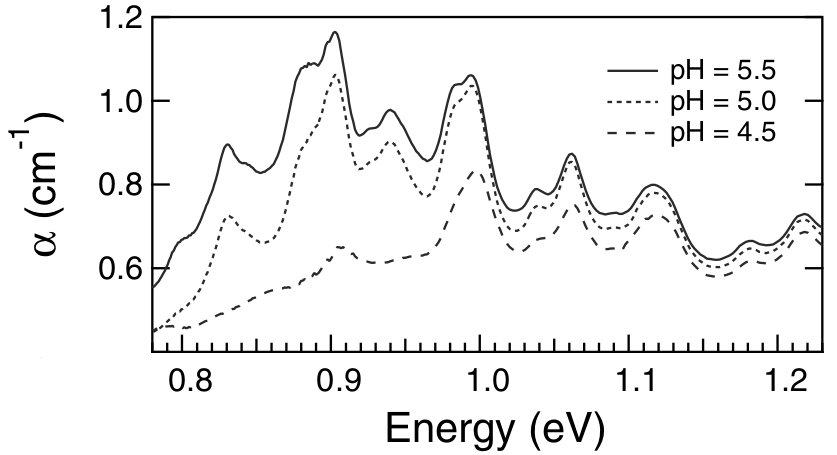
\includegraphics[scale=1.7]{images/chapter_prior_works/ph_effect_gordana_revised}
	\caption{The effect of pH on linear absorption. As the pH reduces from 5.5 to 4.5, absorption peaks at lower photon energies become supressed. This occurs as a consequence of the Burstein-Moss effect, as H$^+$ ions act as dopants that accept electrons. These dopants primarily affect larger-diameter nanotubes, as they exhibit lower binding energies for acceptors in light of their smaller effective masses. Reproduced and modified from Ref.\ \cite{ostojic2004interband}.}
	\label{fig:ph_abs_gordana}
\end{figure}

\begin{figure}[H]
	\centering
	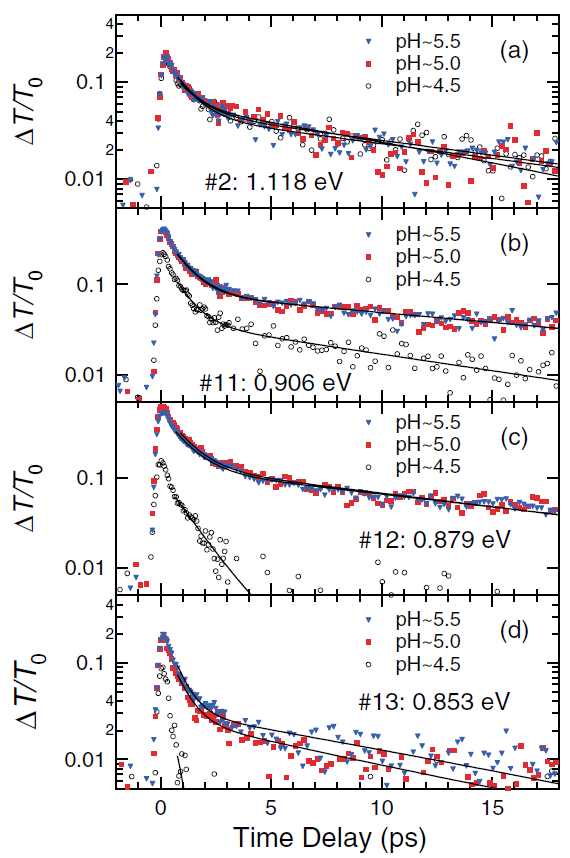
\includegraphics[scale=0.55]{images/chapter_prior_works/dtt_ph_gordana}
	\caption{The effect of pH on the carrier dynamics of nanotubes. Each plot corresponds to a degenerate pump-probe experiment conducted at a specified photon energy. As pH decreases, nanotubes become increasingly doped with positively-charge carriers. This has a larger effect on larger-diameter nanotubes due to their lower acceptor binding energies and lower the Fermi level into the valence band. At lower photon energies, the inter-band recombination process does not appear as the optical resonances associated with this process become supressed. Reproduced and modified from Ref.\ \cite{ostojic2004interband}}
	\label{fig:dtt_ph_gordana}
\end{figure}


\section{Inter-subband Relaxation Dynamics}
Manzoni et al.\ investigated the inter-subband dynamics of SWCNTs using non-degenerate pump-probe measurements with a time resolution of 40 fs. They used two OPAs to generate pump and probe pulses respectively. Furthermore, the sample they studied was a nanotube film made using HiPCo SWCNTs. Figure \ref{fig:abs_manzoni} shows the optical absorption spectrum of this sample along with the specta of the pump pulses used in this study. The sample contains a variety of optical resonances that belong to semiconducting and metallic nanotubes. The spectral regions labeled as EX1, EX2, and EX3 indicate $E_{11}$, $E_{22}$, and $E_{33}$ resonances of semiconducting nanotubes respectively. The region marked as Metallic shows the $E_{11}$ resonances for metallic nanotubes.

\begin{figure}[ht]
	\centering
	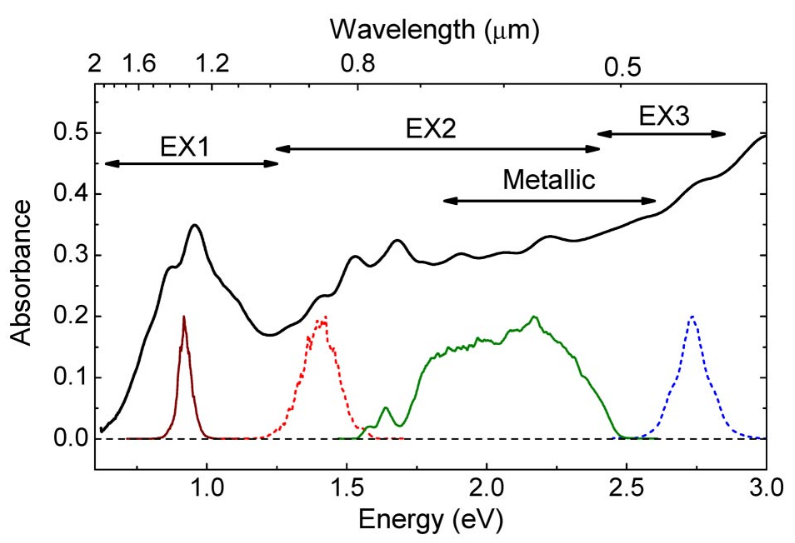
\includegraphics[scale=0.4]{images/chapter_prior_works/abs_manzoni}
	\caption{The black, solid line up top shows the absorption spectrum of HiPCo SWCNT film studied by Manzoni et al. (2005). The spectral regions indicated as EX1, EX2, and EX3 contain the $E_{11}$, $E_{22}$, and $E_{33}$ transitions of semiconducting nanotubes respectively. The region labeled as Metallic contains the $E_{11}$ resonance of metallic nanotubes. The plots shown below represent the spectra of optical pump pulses used to photo-excite the SWCNT sample in this study. Reproduced and modified from Ref.\ \cite{manzoni2005intersubband}.}
	\label{fig:abs_manzoni}
\end{figure}

Depending on the pump and probe photon energies, the observed carrier relaxation dynamics either exhibit photo-induced transsmission or photo-induced absorption. For instance, Figure \ref{fig:e11_pump_manzoni} shows the experimental results obtained when pumping in the EX1 region at 0.92 eV. The differential transmission signal probed at 0.95 eV shows clear signs of photo-bleaching which indicates a finite population of photo-excited carriers. In contrast, the dynamics probed at 2 eV indicate the presence of photo-induced absorption.

Photo-bleaching does not occur due to the fact that the photon energy of the pump is below photon energies of the resonances in EX2. Hence, this photo-induced absorption was interpreted to occur due to an inter-subband transition between a state in the EX1 region and another appropriate state located in EX3 as the energy difference between two such states would be on the order of 2 eV. Additionally, this probe signal at 2 eV exhibits an oscillatory component that was attributed to a radial breathing mode (RBM) of semiconducting CNTs that occurs at a frequency of 259 $\text{cm}^{-1}$. From examining Raman spectra, this indicated that SWCNTs such as (10,3), (11,1), (9,4) and (9,4) were photo-excited in this measurement.


When exciting the SWCNTs at an energy of 2.15 eV in the EX2 region, different dynamics occurred as shown in Figure \ref{fig:e22_pump_manzoni}. Photo-bleaching occurred at the probed photon energy of 0.95 eV. In addition, both photo-induced and transmission and absorption occurred at the probed photon energy of 2.15 eV. The initial photo-bleaching indicates a finite population of $E_{22}$ excitons. Furthermore, the decay occuring afterwards indicates the relaxation from $E_{22}$ to $E_{11}$. This process occurs on a time scale of 150 fs with an associated exponential decay constant of $\sim$40 fs. The photo-induced absorption was again interpreted to occur due to a possible transition between an EX1 state and an EX3. An oscillatory signal was also observed here which was associated with an RBM frequency of 246 $\text{cm}^{-1}$ linked with nanotubes such as (10,3), (9,5), (9,4), and (7,6).


\begin{figure}[H]
	\centering
	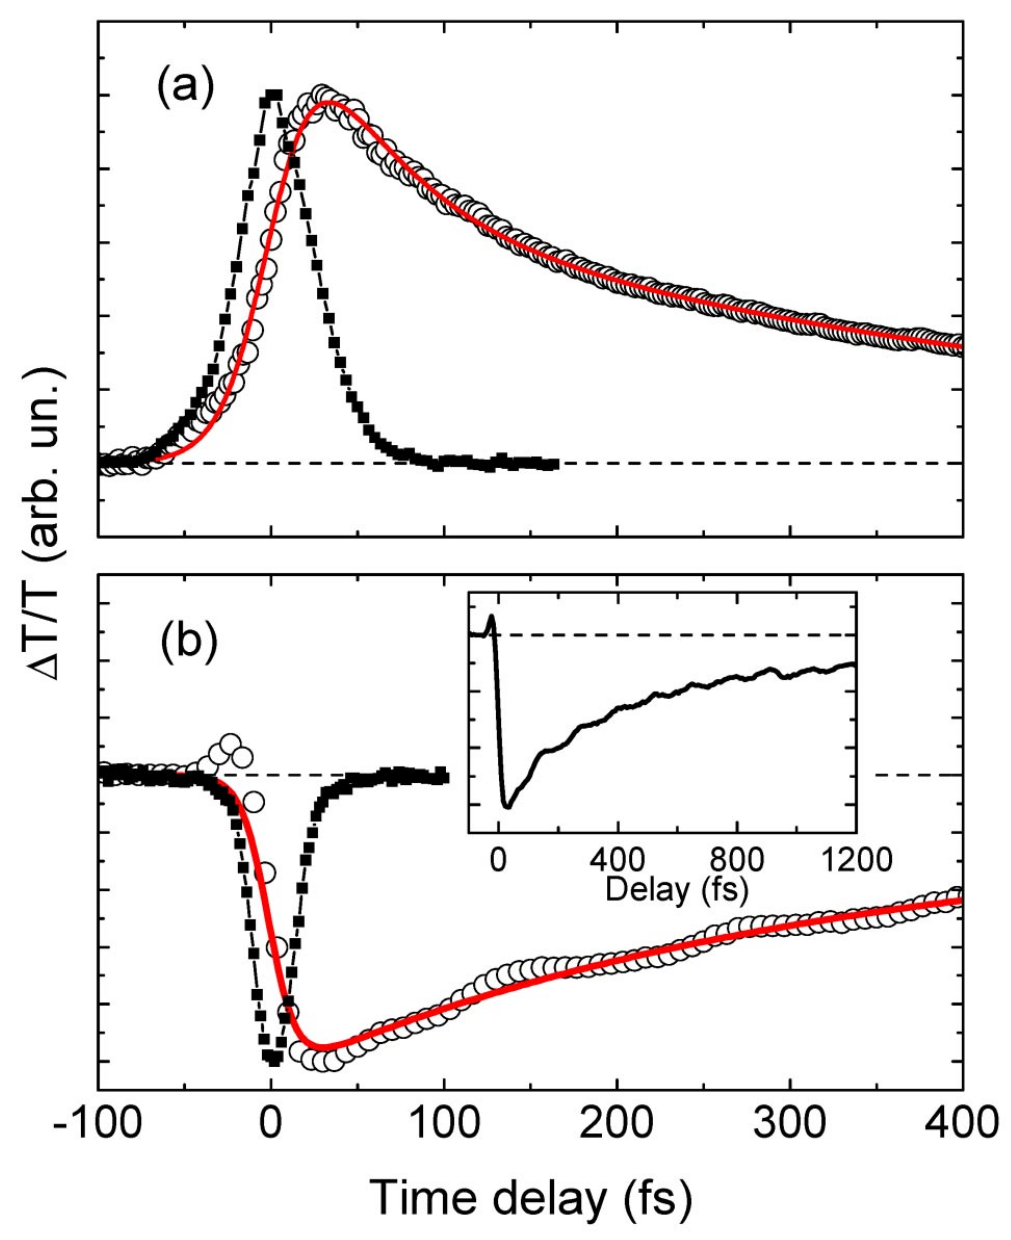
\includegraphics[scale=0.2]{images/chapter_prior_works/e11_pump_probe_manzoni}
	\caption{Carrier relaxation dynamics of SWCNTs photo-excited at 0.92 eV. Under this condition, the two plots correspond to differential transmission probed at 0.92 eV (a) and probed at 2.15 eV (b). The inset figure shows the relaxation measured at 2 eV on a longer time scale. The open circles represent the experimental data, and the solid lines indicate numerical fits to the data. The autocorrelation measurement of the pump pulse is also overlayed on both figures (squares + line). Reproduced from Ref.\ \cite{manzoni2005intersubband}.}
	\label{fig:e11_pump_manzoni}
\end{figure}

\begin{figure}[H]
	\centering
	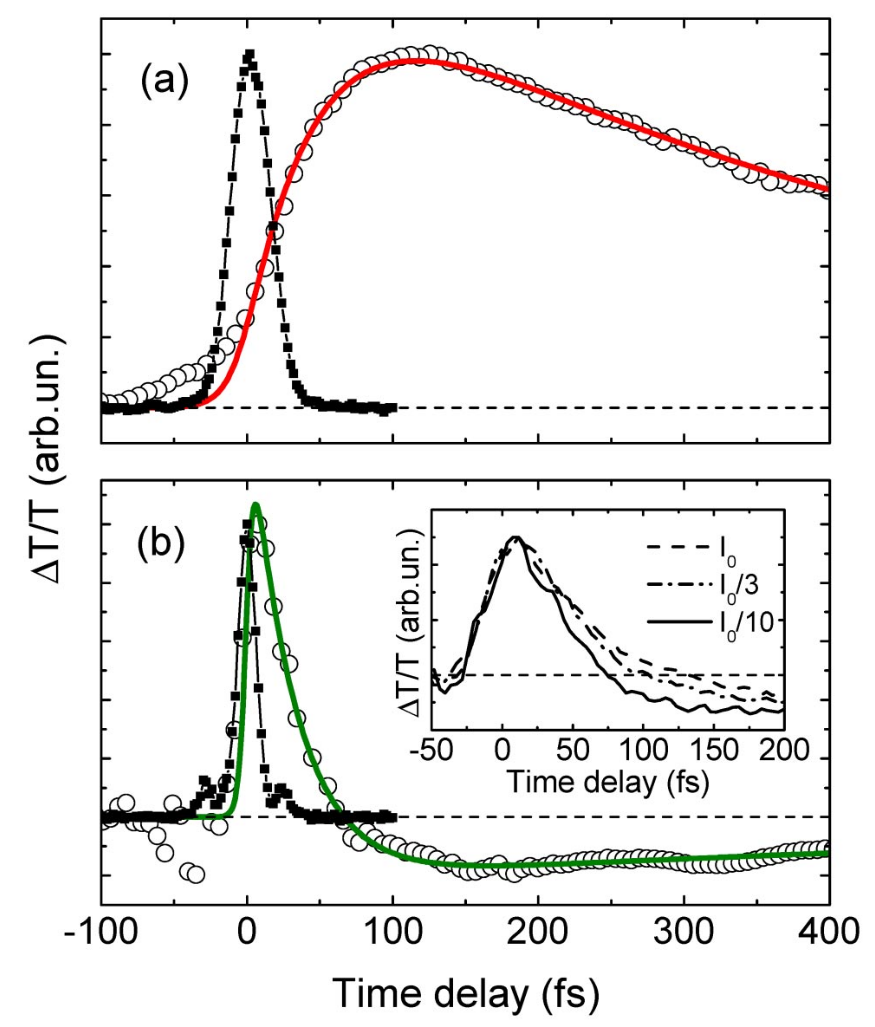
\includegraphics[scale=0.25]{images/chapter_prior_works/e22_pump_probe_manzoni}
	\caption{Carrier relaxation dynamics of SWCNTs photo-excited at 2.15 eV. Under this condition, the two plots correspond to differential transmission probed at 0.95 eV (a) and probed at 2 eV (b). The inset figure shows the pump power dependence measurements of the differential transmission probed at 2 eV. The open circles represent the experimental data, and the solid lines indicate numerical fits to the data. The autocorrelation measurement of the pump pulse is also overlayed on both figures (squares + line). Reproduced from Ref.\ \cite{manzoni2005intersubband}.}
	\label{fig:e22_pump_manzoni}
\end{figure}

Figure \ref{fig:e33_pump_manzoni} illustrates the effect of photo-exciting at 2.75 eV (EX3) and probing at 2.1 eV (EX2). Under these conditions, a small photo-bleaching signal followed by photo-induced absorption occurred. This demonstrated the fast relaxation dynamics from EX3 states into EX1 states. Furthermore, the time constant for this process found to be $\sim$65 fs. Following the previous observations, the photo-induced absorption observed at EX2 also indicated the carrier occupation of EX1 states.

\begin{figure}[ht]
	\centering
	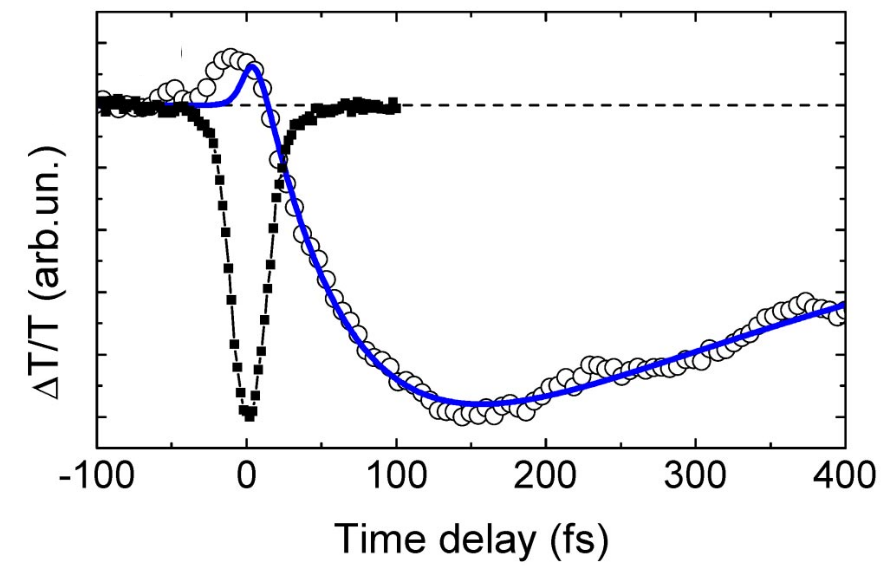
\includegraphics[scale=1.3]{images/chapter_prior_works/e33_pump_e22_probe_manzoni}
	\caption{Carrier relaxation dynamics of SWCNTs photo-excited at 2.75 eV and probed at 2.1 eV. The open circles represent the experimental data, and the solid line indicates a numerical fit to the data. The autocorrelation measurement of the pump pulse is also overlayed on the plot (squares + line). Reproduced from Ref.\ \cite{manzoni2005intersubband}.}
	\label{fig:e33_pump_manzoni}
\end{figure}

Finally, Manzoni et al.\ mentioned that they observed a weak relationship between optical pump intensity and observed recombination dynamics as shown in the inset plot of Figure \ref{fig:e22_pump_manzoni}. At higher pump intensities, the time constant for the exponential decay did not change in a significant fashion. Thus, they did not observe exciton-exciton annihilation in their studies.

\section{The Limits of Exciton-Exciton Annihilation}

Efficient exciton-exciton annihilation \cite{murakami2009existence}.

\begin{figure}[h]
	\centering
	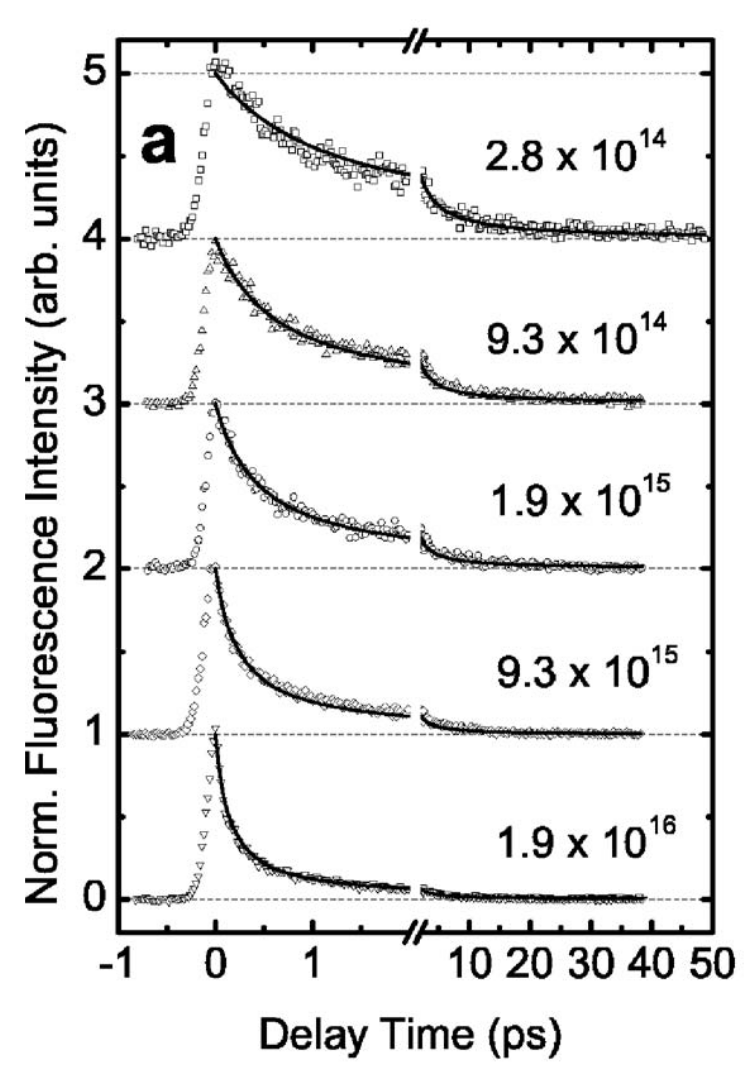
\includegraphics[scale=0.3]{images/chapter_prior_works/pl_valkunas}
	\caption{Reproduced from Ref.\ \cite{valkunas2006exciton}}
\end{figure}

\begin{equation}
\label{eq:exc_annih}
\ce{X + X $\rightarrow$ X},
\end{equation}


%\section{Possible Presence of Bi-excitons and Trions}

%non-degenerate pump-probe. Amplified Ti:sapphire laser operating at 200 KHz and pulse duration of 100 fs. Probe generated using supercontinuum generation in a sapphire crystal. Pump generated using optical parametric amplifier (OPA). Studied a (6,5)-enriched dispersion. Figure \ref{fig:abs_yuma} shows linear absorption spectrum of sample.

%\begin{figure}[ht]
%	\centering
%	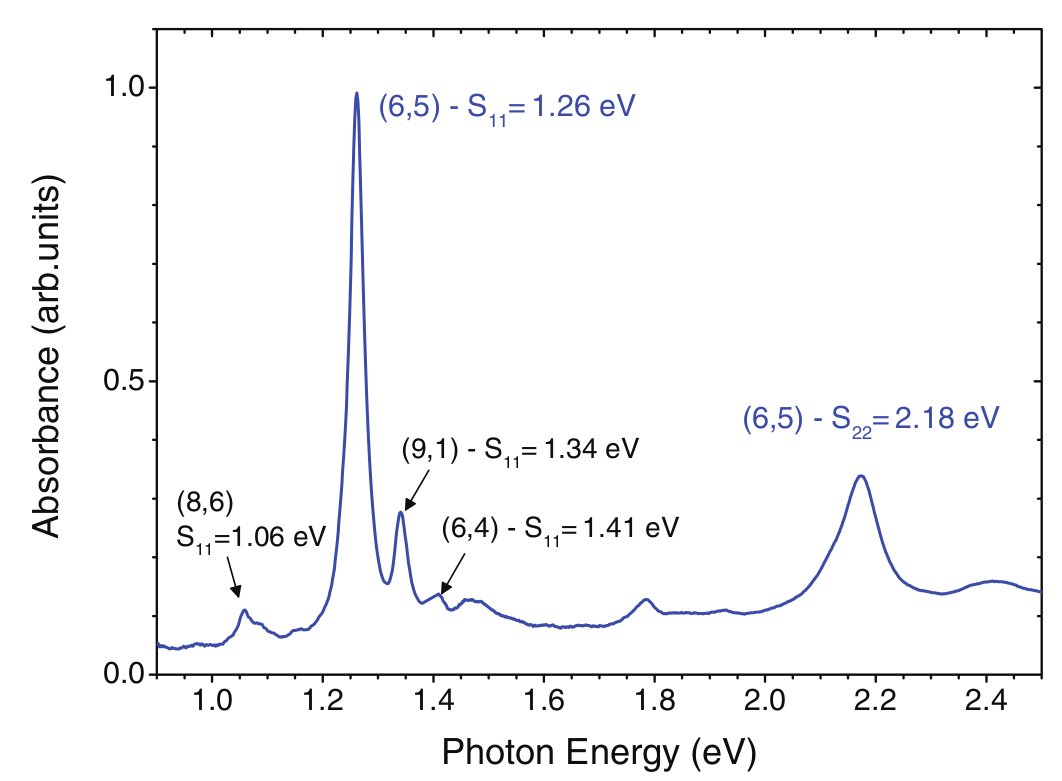
\includegraphics[scale=0.3]{images/chapter_prior_works/abs_yuma}
%	\caption{Slightly different nomenclature. Here, $S_\text{ij} \equiv E_\text{ij}$.  Reproduced from Ref.\ \cite{yuma2013biexciton}.}
%	\label{fig:abs_yuma}
%\end{figure}

%Figure \ref{fig:dtt_yuma} shows experimental data after resonantly exciting $E_{22}$ transition of (6,5) nanotube. Notice photo-bleaching and a blue shift occuring at $E_{11}$ peak. Interpreted as excitons occupying $E_{11}$ states. Charge screening due to Coulomb interactions between excitons blueshifts exciton peak. State that initial sharp decay due to exciton-exciton annihilation.

%Observed photo-induced absorption at 1.13 eV. Attribute this to the formation of biexcitons. Provided additional evidence by pumping at and below $E_{11}$. When pumping below $E_{11}$, photo-induced absorption at 1.13 eV recedes. When pumping $E_{11}$ resonantly, photo-induced absorption becomes more significant indicating that it may be directly associated with (6,5). Carrier dynamics at $E_{11}$ and bi-exciton appear to be correlated with each other.

%\begin{figure}[ht]
%	\centering
%	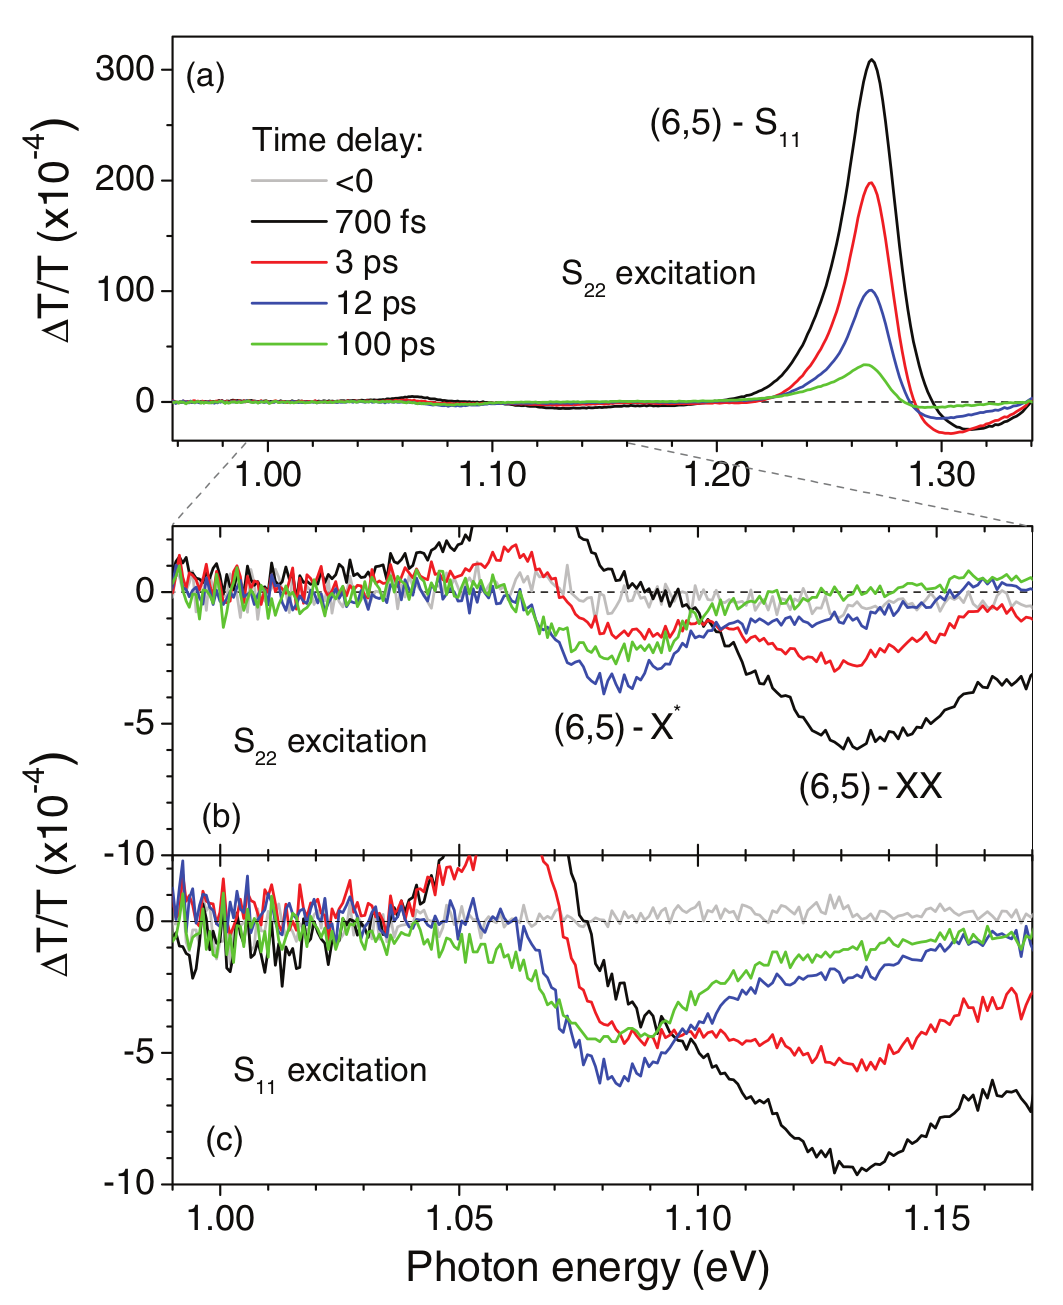
\includegraphics[scale=0.3]{images/chapter_prior_works/dtt_yuma}
%	\caption{{\color{red} UNFINISHED} Reproduced from Ref.\ \cite{yuma2013biexciton}.}
%	\label{fig:dtt_yuma}
%\end{figure}


%Exciton-Exciton annihilation \cite{valkunas2006exciton, yuma2013biexciton}.
%They also show that exciton-exciton annihilation occurs over a time scale such that it is hard to reach Mott densitty of excitons where excitons immediately dissociate to form plasma of free carriers. These a
%Apparently, excitons dissociate into free electron-hole pairs before recombination occurs \cite{kumamoto2014spontaneous}.




\section{Summary}
